\documentclass{cranfieldChart}

\bibliography{biblio.bib} 


\begin{document}

\maketitle{About report \& latex}{Thibaud Levasseur}{School of Aerospace, Transport and Manufacturing}{Software Engineering for Technical Computing }{cover.png}

\begin{abstract}
This is the abstract of my very important report about that lab we did that day, and I have tons of results to comment. 
\end{abstract}

\newpage
\tableofcontents
\newpage
\listoffigures
\newpage
\listoftables
\newpage
\section{Stuff I tried to implement}
\subsection{First thing}
This is a section.
\subsubsection{Details}
This is subsection.
\subsubsection{More details}
This is another subsection.
\subsection{Second thing}
\subsection{Third thing}
\newpage
\section{Result}
\subsection{Of the first thing}
Those results are in the figure \ref{resuts}. The caption is on the top of it !
\begin{table}[!h]
	\centering
	\caption{My results}
	\label{resuts}
	\begin{tabular}{lllll}
		& a  & b  & c & d \\
		& e & f & g & h \\
		& i & j & k & l \\
		& m & n & o & p
	\end{tabular}
\end{table}
\subsection{Of the second thing}
Here is a picture of a tree (see figure \ref{tree}). It has the caption under it !
\begin{figure}[!h]
	\centering
	
	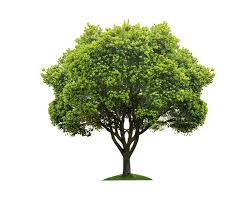
\includegraphics{ressources/tree.jpg}
	\caption{A big tree}
	\label{tree}
\end{figure}
\subsection{Of the third thing}
I am so sorry, I forgot.
\paragraph{}
Maybe I could remember in that new paragraph what i read in that book : "1+1=2" \autocite{ref0}

\newpage
\section{Conclusion}
Done ! See you for the prom !

\newpage

\printbibliography



\end{document}